\setlength{\parindent}{2em} %首行缩进

\section{實驗目的:}
\begin{enumerate}[label=\arabic*.]
  \item 利用 PCR 技術,複製大腸桿菌轉型實驗中的DNA。
  \item 觀察並比較轉型成功與未成功的細菌 DNA 電泳結果。

\end{enumerate}



\section{實驗步驟:}

\subsection*{實驗器材}

\begin{multicols}{2}
  \begin{enumerate}[label=\arabic*.]
    \item polymerase reagent(20μL)
    \item primer mixture(20μL)
    \item 大腸桿菌轉形實驗中含藍、白菌落的培養基
    \item 500μL 的 PCR tube x2
    \item P20
    \item Eppendorf
    \item PCR machine
    \item 電泳儀
    \item 電源供應器
    \item Agarose gel
    \item 電泳 buffer
    \item Light box
    \item 離心機
  
  \end{enumerate}  
\end{multicols}

\subsection*{步驟}

\begin{enumerate}[label=\arabic*.]
  \item 取兩個 500μL 的 PCR tube 並用標示 W 和 B,各自加入 10μL 的 polymerase reagent 和 10μL 的 primer mixture,再pipetting 得到 PCR sample。
  \item 用兩個 P200/P20 的 tip 分別沾取培養基中的藍色與白色菌落,再分別加入標示 W 和 B 的 PCR tube,與 PCR sample 均勻混合。(若混合後氣泡過多或液體殘留在管壁,可先離心再進行下一步驟)
  \item 將標示 W 和 B 的 PCR tube 放到 PCR machine 中反應 40 分鐘。
  \item 從 W 和 B 兩管各用 pipette 取 10μL 到 eppendorf 的蓋子上,再分別取 2μL 的 loading buffer 與之混合,最後 load 到 agarose gel 裡面,以 140V 電泳 15 分鐘。
  \item 將跑完的 agarose gel 放到 light box 觀察。
  
\end{enumerate}



\newpage
\section*{實驗結果及討論:}
\subsection*{結果}
\begin{figure}[H]
\centering
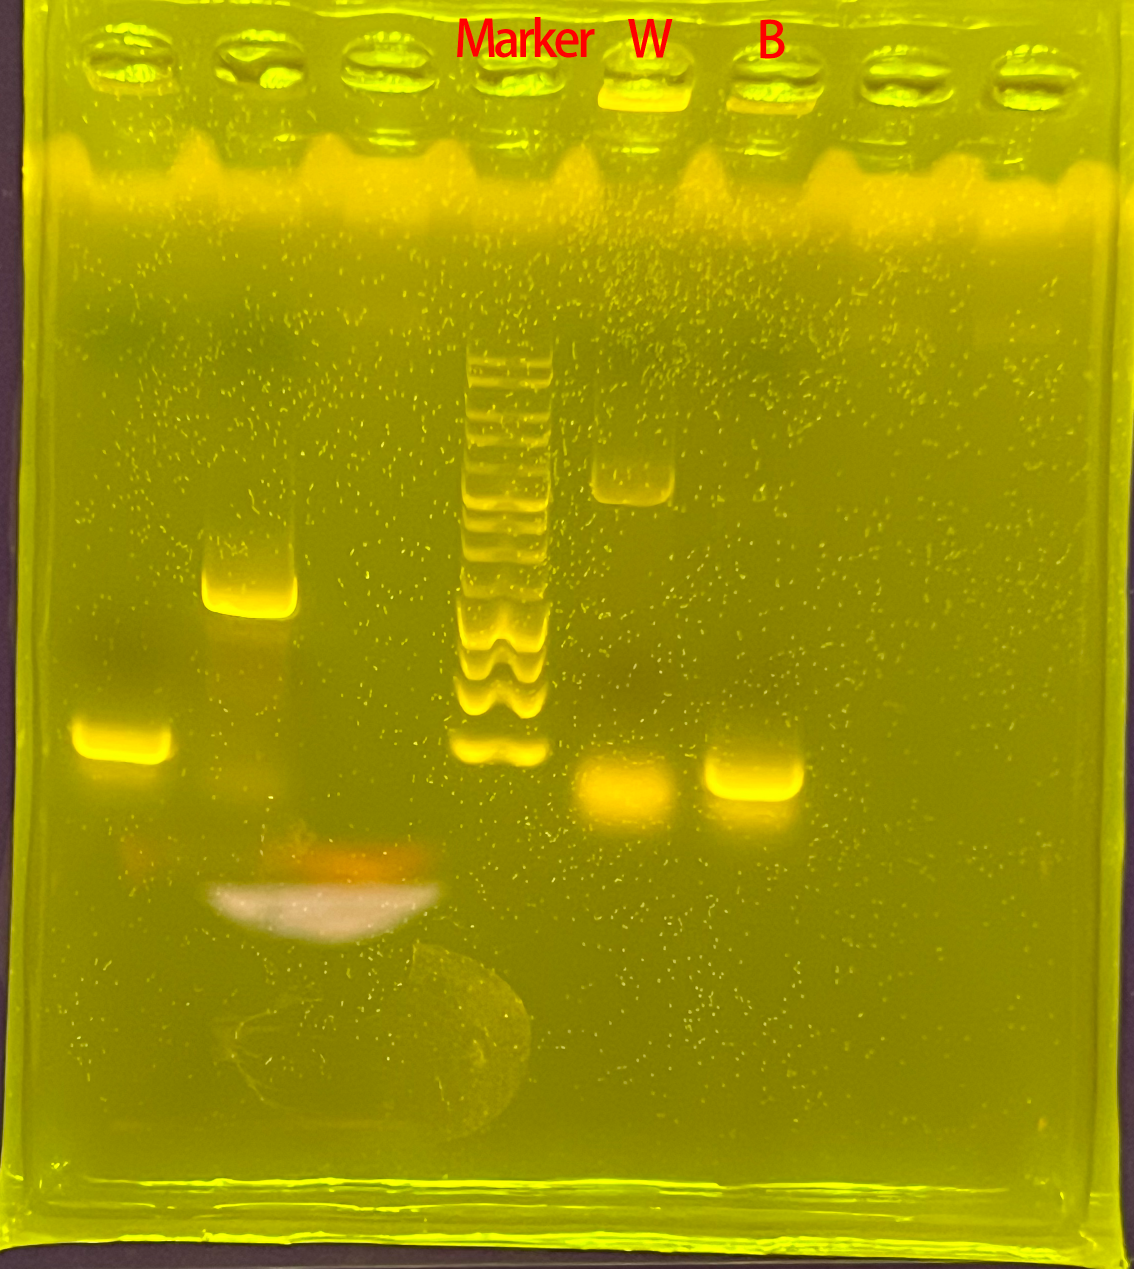
\includegraphics[width=0.5\textwidth]{paste_src/rt1.png}
\end{figure}

\begin{enumerate}[label=\arabic*.]
  \item 白色菌落 (W組) 在 3-4kbp 與有明顯亮帶,於 250bp 以下有較模糊的亮帶。
  \item 藍色菌落 (B組) 僅在 250bp 以下有明顯亮帶。
\end{enumerate}


\subsection*{實驗討論}


\dsc 電泳結果的意義 
\begin{enumerate}[label=\arabic*.]
  \item 白色菌落的 colony 有成功 insert,其 DNA 分子量較大,電泳時移動速度較慢;藍色菌落的 colony 未成功 insert,其 DNA 分子量較小,電泳時移動速度較快。
  \item 白色菌落在對藍色菌落的亮帶處也有模糊的亮帶,推測是因為沾取到部分沒有 insert 成功的 colony 造成。
  \item 藍色與白色菌落的 colony 皆為環狀 DNA ,其分子量都比對應到的 Marker 分子量大。

\end{enumerate}


\dsc 進行PCR實驗後進行核酸電泳如果有實驗上的誤差,可能造成的原因為何?

\begin{enumerate}[label=\arabic*.]
  \item PCR反應失敗: 如果PCR反應本身存在問題,例如缺乏DNA模板、Primer設計不當、PCR條件不準確等,則核酸電泳的結果可能是無產物或者不正確的產物。\
  \item 樣品污染: 樣品可能受到DNA或RNA污染,這可能來自實驗室環境、實驗者、或者之前的實驗。污染會導致其他產物出現在膠片中。
  \item 電泳條件不當: 選擇不當的電泳條件(例如電壓、運行時間)可能導致產物的模糊或者過度擴散。這可能使不同大小的DNA片段難以區分。
  \item 樣品負載量不均: 如果樣品負載量不均,則可能在電泳圖譜中看到強度差異明顯的條帶,這可能會影響樣品的比較和分析。
  \item DNA量不足: 如果PCR反應的起始DNA量太少,則可能難以在電泳中檢測到目標產物。這可能發生在樣品提取或者PCR反應的早期階段。
  \item 引物選擇: Primer的設計可能影響PCR產物的specificity。如果Primer與非特異的DNA結合,則可能在電泳中觀察到額外的亮帶。
  \item 電泳環境: 電泳室的環境條件,例如溫度和緩衝液,可能對電泳結果產生影響。環境條件的不穩定可能導致結果的不一致性。
  \item 膠體質量: 使用老化、變質或者不適當的瓊脂糖膠可能導致電泳結果不準確。
\end{enumerate}


\dsc 我們這組實驗的誤差來源?如何減少本次實驗所造成的誤差與錯誤?

與膠片上的另外一組相比,我們這組白色菌落的亮帶較不清晰,而且在250bp處還有模糊的亮帶,可知樣品可能受到DNA或RNA污染,而汙染的由來可能是我們在取白色菌落的時候,有沾染到其他東西,或者在呼吸的過程中有引入汙染物。在取樣及把樣品加入PCR tube的時候應該更加迅速且準確,以避免樣品受到汙染。

\dsc qPCR的應用

\begin{enumerate}[label=\arabic*.]
  \item 基因表達分析: qPCR用於量化特定基因的mRNA水平,進行基因表達研究。這可以幫助研究者了解基因在不同條件下的表達模式,探討生物學過程和疾病的機制。
  \item 基因型分析: qPCR可用於檢測和定量DNA序列的存在,從而進行基因型分析。這在基因組學研究和遺傳學研究中具有重要意義,例如檢測基因突變、基因多態性等。
  \item 病原體檢測: qPCR被廣泛應用於檢測和定量病原體,如細菌、病毒、真菌等。這對於臨床診斷、疾病監測和食品安全檢測都具有重要的意義。
  \item 病毒量化: 在病毒學研究中,qPCR可用於量化病毒的基因體或RNA,並評估病毒複製和感染的程度。但病毒的RNA 需要先被反轉錄酶(reverse transcriptase)反轉錄回DNA才可進行PCR,故又稱為RT-PCR。
  \item 藥物研發: 在藥物研發過程中,qPCR可用於評估潛在藥物對特定基因的影響,進行基因表達標記物的篩選,並評估藥物的效能。
  \item 生態學和環境研究: qPCR可用於環境樣品中的微生物群體和基因的定量分析,有助於了解生態系統中的微生物多樣性和生態過程。
  \item 轉基因植物檢測: qPCR可以檢測和定量轉基因植物中外源基因的存在和表達,確保農作物品質和生態安全。
\end{enumerate}

\newpage

\dsc Real-time PCR介紹

\begin{itemize}[leftmargin=0cm,]
  \item[] 目的:除了PCR增加目標片段DNA作用,利用螢光物質與DNA片段結合的效果,藉由偵測濃度,達到定量效果。
  \item[] 目前主要分為TaqMan與SYBR green兩種
\end{itemize}

\begin{table}[h]
\centering
\setlength{\abovecaptionskip}{0cm} % 调整caption间距
\begin{tabular}{cp{6cm}p{6cm}}
\toprule
方式&SYBR green&TaqMan\\

\midrule
原理&藉由螢光染劑對雙股DNA有較高親和力的效果,達成PCR過程中螢光強度會隨著cycle數目增加的定量方式。&藉由DNA探針上兩個螢光基團,分別為紅綠,當兩基團較接近時,紅色螢光因為波長較長造成綠色螢光無法被偵測,而PCR過程中,兩基團隨著DNA合成而遠離,綠色螢光基團則可被偵測,達成定量目的。\\
\midrule
優點&較便宜、降低實驗設計的複雜度&較為準確\\
\midrule
缺點&比起TaqMan方式有較高的誤差&設計DNA探針較為複雜、昂貴\\
\bottomrule


\end{tabular}\end{table}





%\bibliography{bibfile} 
%\bibliographystyle{unsrt}
